\section{Hyperparameter Search}

The tokenizer grid described in the REMI+ section is not treated here as an xLSTM hyperparameter search. It is a representation-selection stage: it measures how different MidiTok configurations preserve MIDI content under tokenization and decoding. The xLSTM experiments then test which model size, batch size, schedule, and tokenizer representation are useful for the downstream next-token objective.

The W\&B run chronology is important for interpreting these results. The first finished runs were warm-up experiments tagged \texttt{batch\_size\_sweep} on April 30--May 1, 2026. The learning-rate runs are tagged \texttt{lr\_sweep} and were run on May 11--12. The tokenizer-condition runs are tagged \texttt{tok\_sweep} and were run on June 20--21. The refined tokenizer--batch runs are tagged \texttt{best\_tok\_sweep} and were run on June 21--22. The medium follow-up was run on June 28 without a sweep tag. This sequence matches the practical workflow: first verify that the training loop behaves sensibly, then tune optimization, then compare representations, then use the best observed setup for a larger model.

\subsection{Warm-Up Scale and Batch Runs}

The first runs were deliberately small in scope. They used tokenizer 11, the same train/validation split, block size 1024, and three epochs. The goal was not to select a final model, but to understand whether the xLSTM implementation, data loading, validation loop, and checkpointing behaved plausibly before spending more GPU time.

\begin{figure}[htbp]
	\centering
	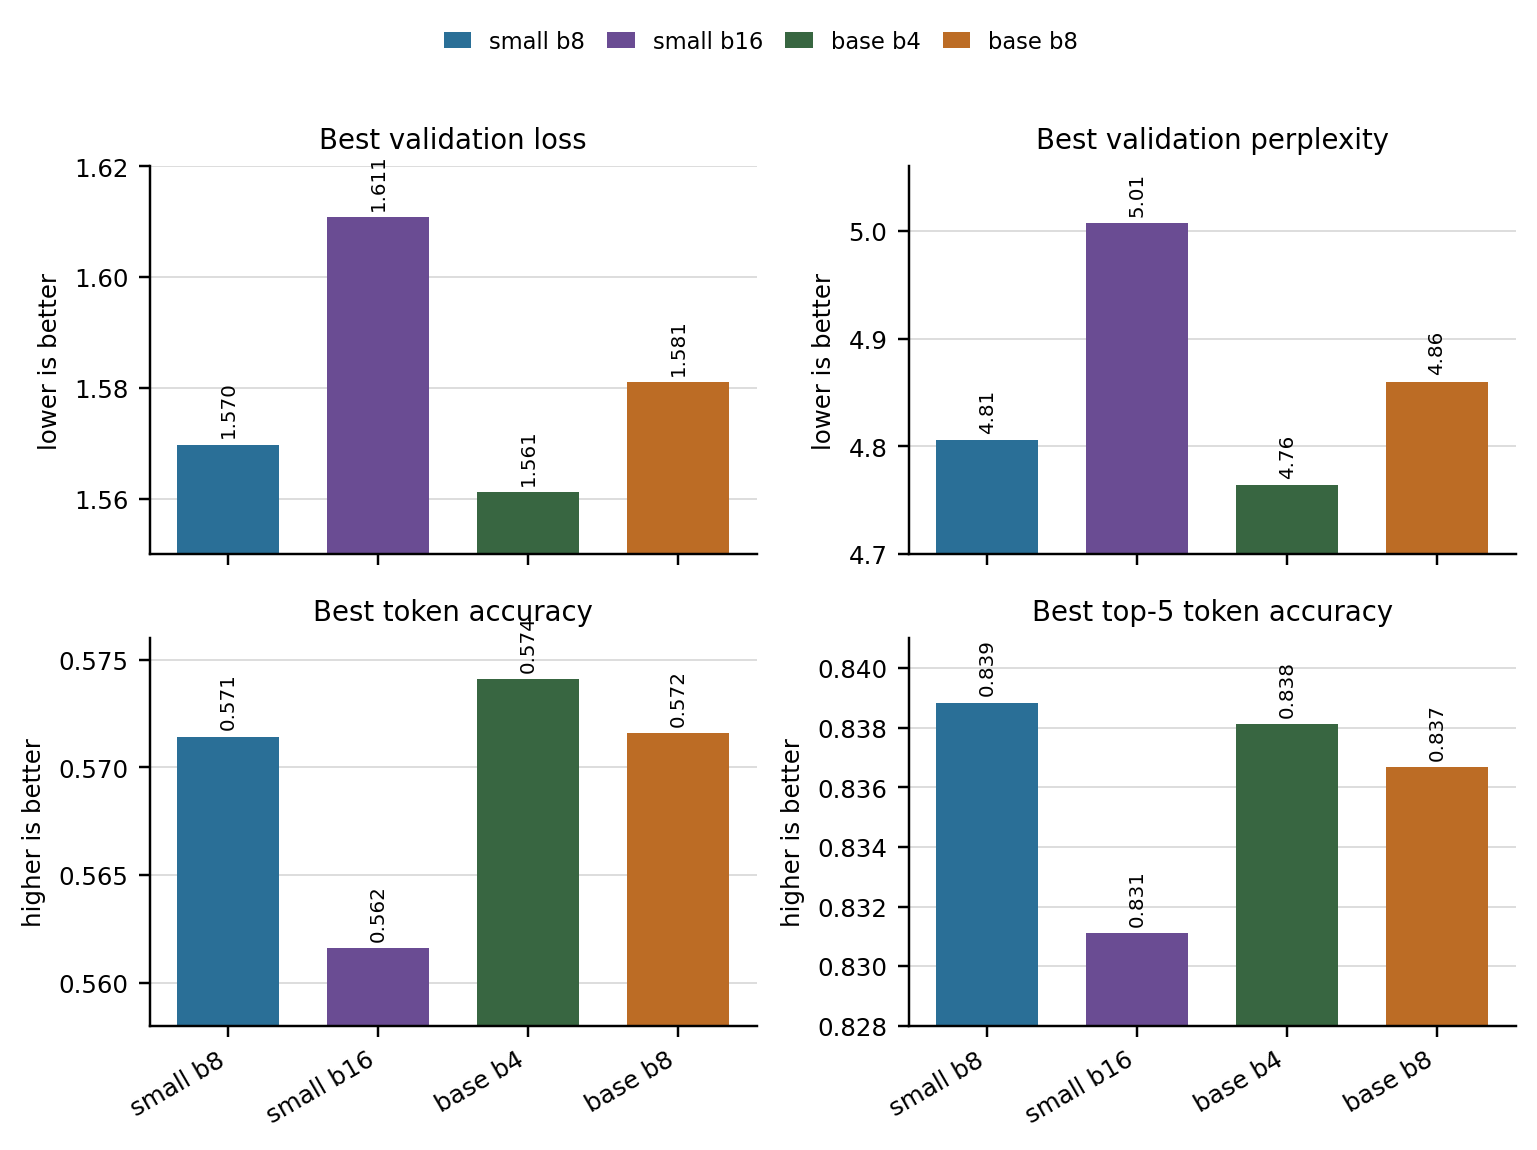
\includegraphics[width=0.82\textwidth]{figures/xlstm_warmup_scale_best_val_metrics.png}
	\caption{The panels compare best validation loss, best validation perplexity, best token accuracy, and best top-5 token accuracy, with each run keeping the same color across all panels. These runs were used to check basic training behavior before larger sweeps.}
	\label{fig:xlstm-warmup-sweep}
\end{figure}

The warm-up results gave two useful signals. First, the base model was a better default for the next experiments than the small model: the base batch-4 run reached 1.5611 validation loss, while the small batch-8 run reached 1.5698 and the small batch-16 run reached 1.6109. Second, batch size 8 was a practical compromise. Batch size 4 gave the best warm-up validation loss, but it doubled the optimizer steps per epoch and therefore also changed wall-clock cost and update count. Batch size 8 kept the base model affordable while still producing a reasonable baseline. For that reason, the learning-rate sweep fixed the base model and batch size 8 rather than immediately chasing the best warm-up scalar.

\subsection{Learning-Rate Sweep}

The learning-rate sweep was the first controlled training hyperparameter sweep. It kept tokenizer 11, the base xLSTM, batch size 8, block size 1024, and the same three-epoch budget fixed. This avoided confounding schedule comparisons with different model capacities, tokenizers, or numbers of optimizer steps per epoch.

\begin{figure}[htbp]
	\centering
	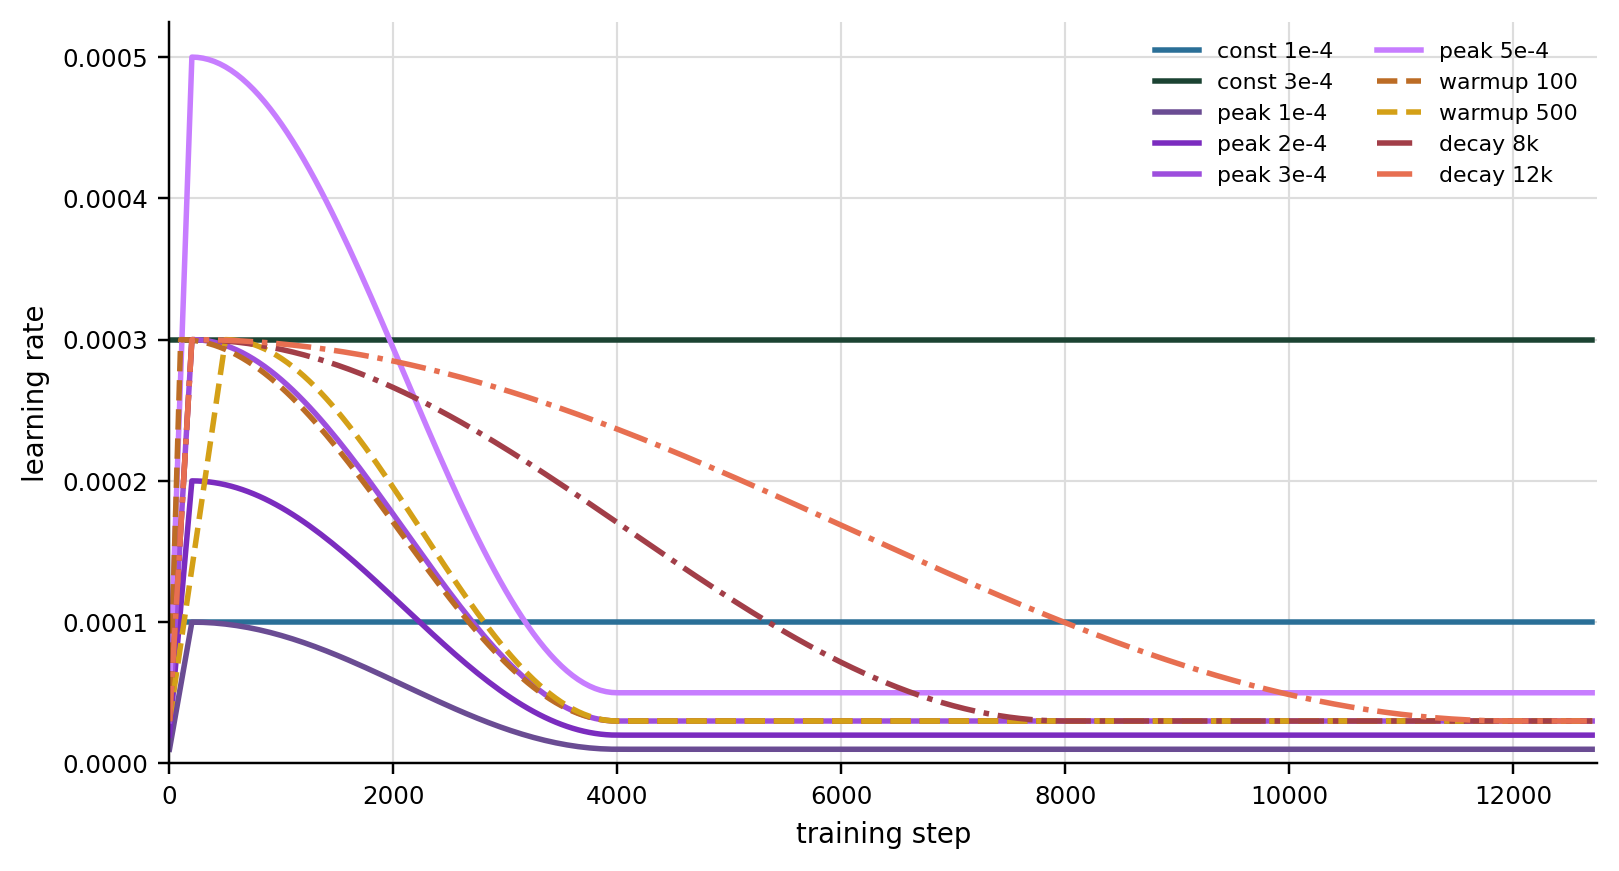
\includegraphics[width=0.90\textwidth]{figures/xlstm_lr_schedulers_sweep.png}
	\caption{Learning-rate schedules used in the tokenizer-11 LR sweep for the base xLSTM with batch size 8, block size 1024, and three epochs. Curves are reconstructed from the resolved training configurations; the corresponding validation summaries are reported in Table~\ref{tab:xlstm-lr-sweep}.}
	\label{fig:xlstm-lr-sweep}
\end{figure}

\begin{table}[htbp]
	\centering
	\scriptsize
	\resizebox{\textwidth}{!}{%
		\begin{tabular}{lrrrrr}
			\toprule
			Learning-rate condition & Best step & Best val. loss  & Best val. ppl.  & Best val. acc.  & Best val. top-5 acc. \\
			\midrule
			\texttt{constant\_1e-4} & 12000     & \textbf{1.5759} & \textbf{4.8349} & \textbf{0.5722} & \textbf{0.8365}      \\
			\texttt{decay\_8000}    & 7000      & 1.5891          & 4.8995          & 0.5695          & 0.8354               \\
			\texttt{decay\_12000}   & 7000      & 1.5893          & 4.9002          & 0.5719          & 0.8356               \\
			\texttt{constant\_3e-4} & 6000      & 1.5895          & 4.9013          & 0.5720          & 0.8342               \\
			\texttt{peak\_5e-4}     & 7000      & 1.5907          & 4.9072          & 0.5687          & 0.8341               \\
			\texttt{warmup\_500}    & 11000     & 1.6007          & 4.9564          & 0.5643          & 0.8317               \\
			\texttt{warmup\_100}    & 12000     & 1.6141          & 5.0236          & 0.5624          & 0.8304               \\
			\texttt{peak\_3e-4}     & 12000     & 1.6179          & 5.0424          & 0.5615          & 0.8304               \\
			\texttt{peak\_2e-4}     & 12000     & 1.6398          & 5.1541          & 0.5540          & 0.8250               \\
			\texttt{peak\_1e-4}     & 12000     & 1.8434          & 6.3179          & 0.5094          & 0.7831               \\
			\bottomrule
		\end{tabular}
	}
	\caption{Learning-rate sweep on tokenizer 11 with batch size 8. All rows use the same train/validation split and three-epoch budget.}
	\label{tab:xlstm-lr-sweep}
\end{table}

The constant \(10^{-4}\) run was the best condition inside this tokenizer-11 sweep, while the very low \(10^{-4}\) peak schedule was clearly under-trained. This result was useful, but it was not the end of the search: it was still tied to tokenizer 11, which had only been selected by the tokenizer-only autotune criterion. The next question was whether a representation that looked worse or longer at the tokenizer level could be easier for the model to learn.

\subsection{Tokenizer Sweep}

The tokenizer sweep moved from optimization tuning to representation testing. It trained the base model with batch size 8 across the strongest tokenizer candidates from the REMI+ autotune stage, including chord-enabled variants. This sweep answers a different question from the tokenizer grid in the previous section. The tokenizer grid asks how faithfully a configuration preserves MIDI under tokenization and decoding; the downstream tokenizer sweep asks how well the xLSTM learns the resulting token stream.

\begin{figure}[htbp]
	\centering
	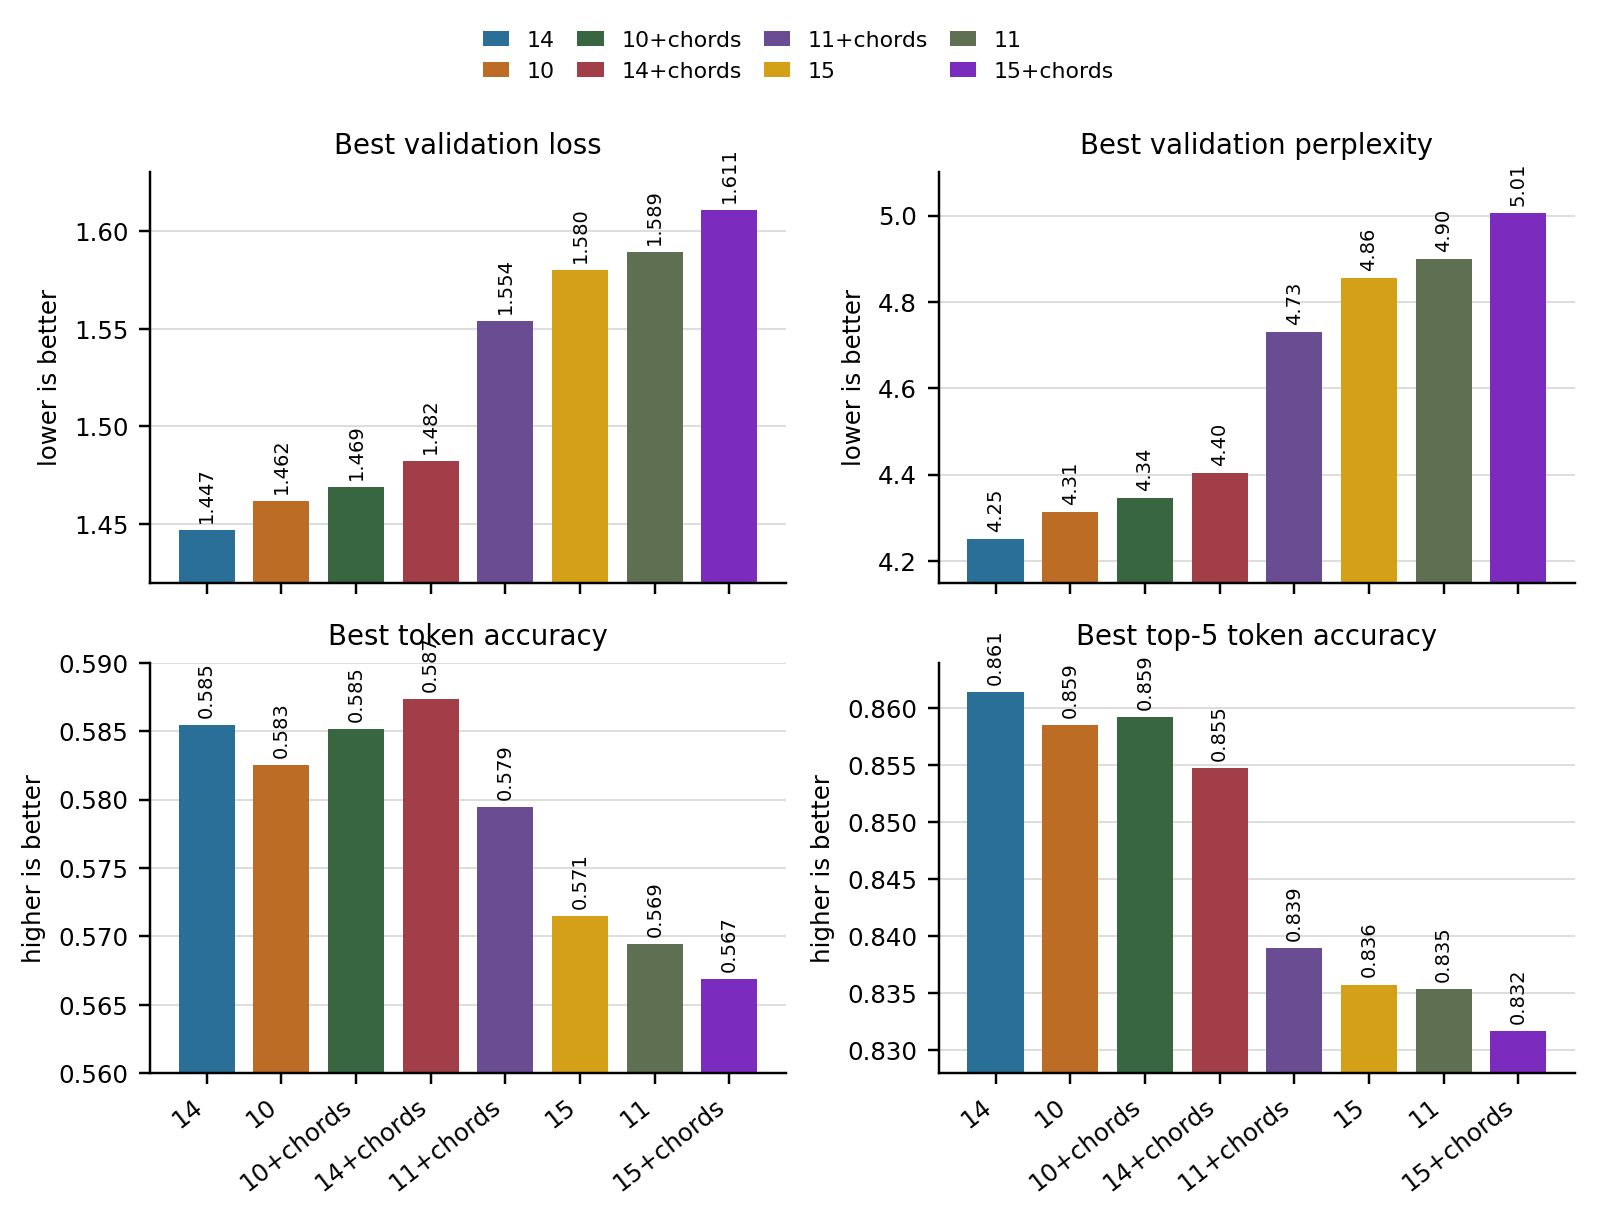
\includegraphics[width=0.88\textwidth]{figures/xlstm_tokenizer_sweep_val_metrics.png}
	\caption{Downstream tokenizer-condition sweep with the base xLSTM, batch size 8, block size 1024, and three training epochs. The panels compare best validation loss, best validation perplexity, best token accuracy, and best top-5 token accuracy. Each tokenizer condition keeps the same color across all panels. This figure uses the exported summaries in \texttt{experiments/xlstm-base-tokenizer-batch-sweep-sched-decay-8000}.}
	\label{fig:xlstm-tokenizer-sweep}
\end{figure}

\begin{table}[htbp]
	\centering
	\scriptsize
	\resizebox{\textwidth}{!}{%
		\begin{tabular}{lrrrrrr}
			\toprule
			Condition                & Vocab. & Steps/epoch & Best val. loss  & Best val. ppl.  & Best val. acc.  & Best val. top-5 acc. \\
			\midrule
			\texttt{tok\_14}         & 646    & 4858        & \textbf{1.4471} & \textbf{4.2507} & 0.5854          & \textbf{0.8614}      \\
			\texttt{tok\_10}         & 598    & 4834        & 1.4619          & 4.3144          & 0.5825          & 0.8586               \\
			\texttt{tok\_10\_chords} & 612    & 4858        & 1.4690          & 4.3447          & 0.5852          & 0.8592               \\
			\texttt{tok\_14\_chords} & 660    & 4858        & 1.4823          & 4.4030          & \textbf{0.5874} & 0.8548               \\
			\texttt{tok\_11\_chords} & 612    & 4255        & 1.5541          & 4.7309          & 0.5795          & 0.8390               \\
			\texttt{tok\_15}         & 646    & 4255        & 1.5801          & 4.8554          & 0.5715          & 0.8358               \\
			\texttt{tok\_11}         & 598    & 4235        & 1.5891          & 4.8995          & 0.5695          & 0.8354               \\
			\texttt{tok\_15\_chords} & 660    & 4255        & 1.6106          & 5.0057          & 0.5668          & 0.8317               \\
			\bottomrule
		\end{tabular}
	}
	\caption{Tokenizer conditions evaluated as downstream xLSTM training conditions.}
	\label{tab:xlstm_runs}
\end{table}

This sweep changed the interpretation of the tokenizer-only result. Tokenizer 11 remained the winner of the tokenizer autotune score, but tokenizer 14 was clearly better for downstream validation loss. Tokenizer 14 has a larger vocabulary and more training chunks than tokenizer 11, because it disables program-change tokens and enables rests, but the base xLSTM predicted it more successfully. The result suggests that compactness alone was not the right criterion for model training. It also showed that chord tokens were not uniformly beneficial: they improved tokenizer 11 relative to tokenizer 11 without chords, but hurt the stronger tokenizer 14 condition.

\subsection{Refined Tokenizer--Batch Sweep}

After the tokenizer sweep, the search was narrowed to the two strongest tokenizer families, 14 and 10. The refined \texttt{best\_tok\_sweep} runs crossed those tokenizers with batch sizes 4, 8, and 16, using the same base model and the same warmup--cosine schedule. This was the point where batch size became a tuning variable again, but only after the representation search had identified stronger candidates than tokenizer 11.

\begin{figure}[htbp]
	\centering
	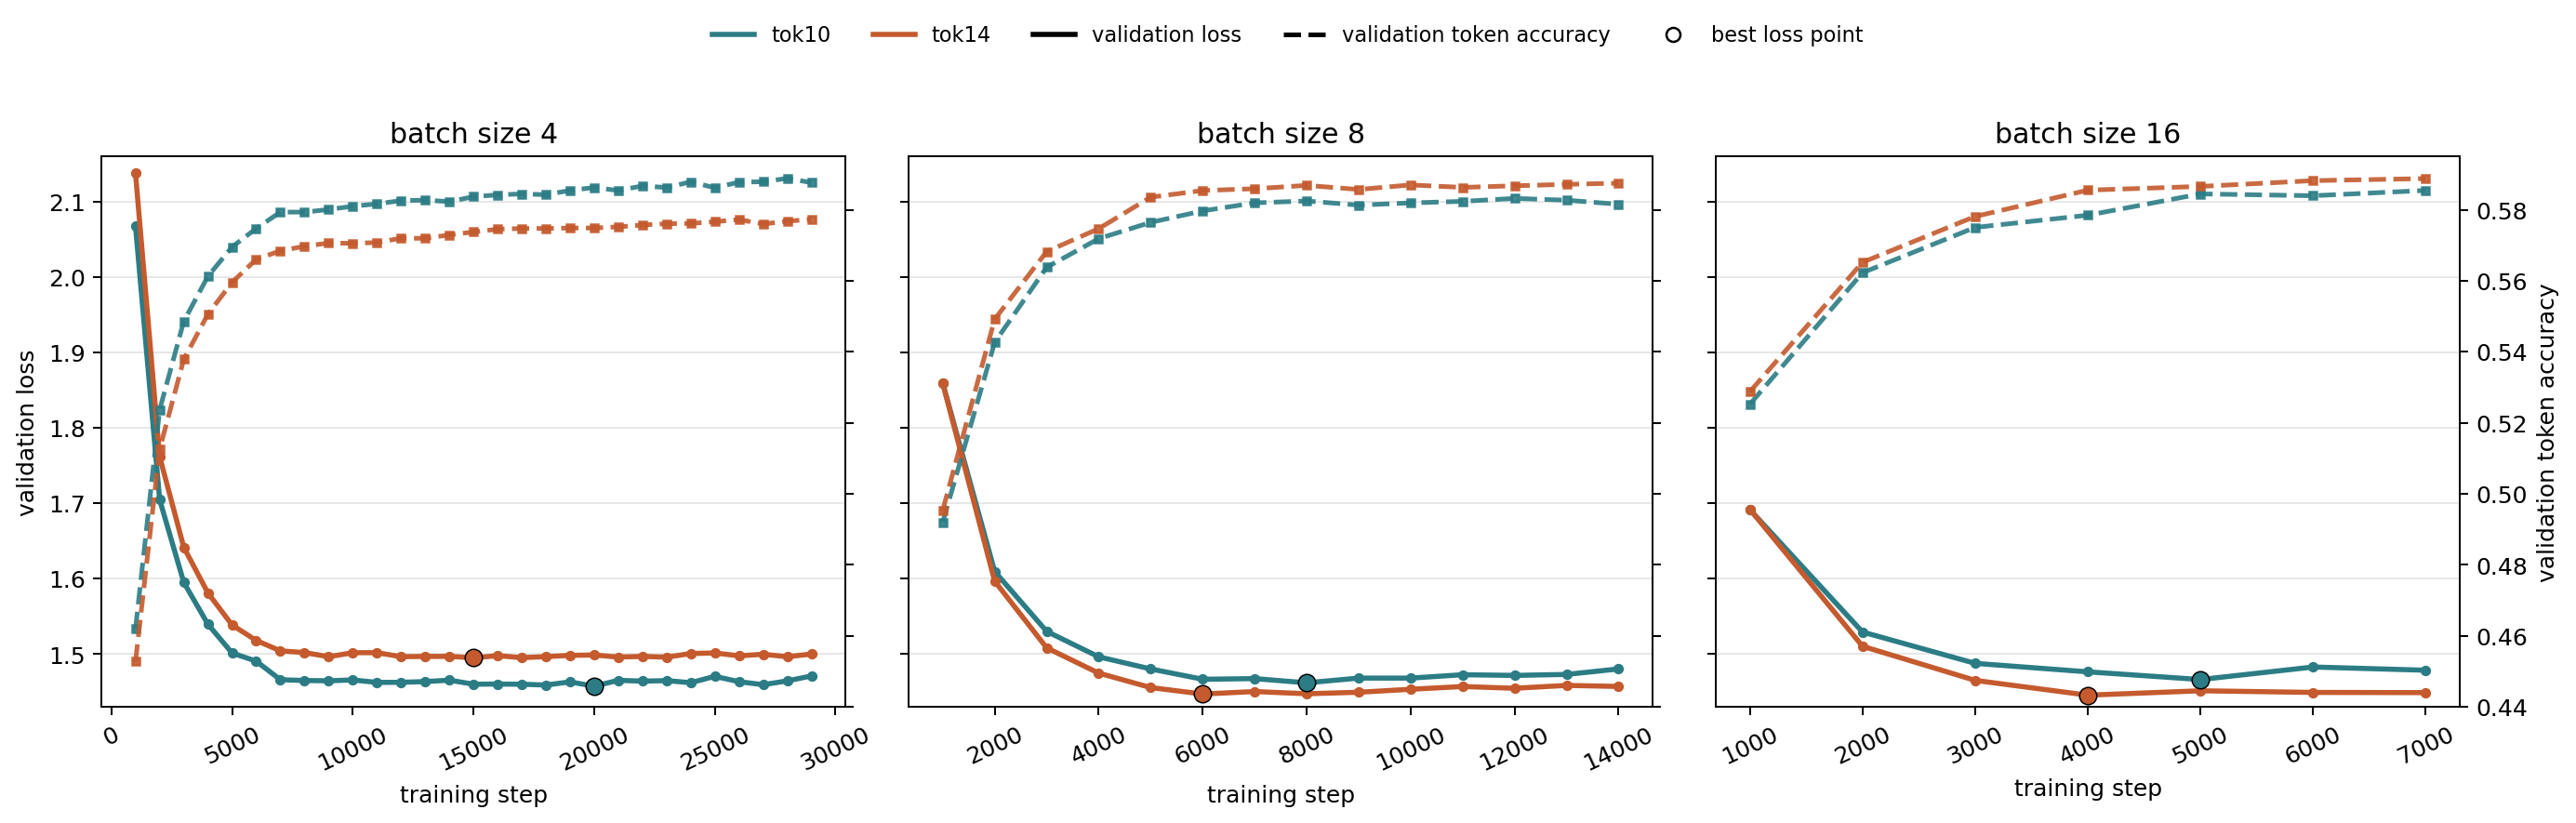
\includegraphics[width=0.90\textwidth]{figures/xlstm_best_tok_sweep_candidate_val_loss_acc.png}
	\caption{Each panel fixes the batch size and compares tokenizer 10 against tokenizer 14; solid lines show validation loss, dashed lines show validation token accuracy, and outlined markers identify the best validation-loss point for each run.}
	\label{fig:xlstm-base-candidate-curves}
\end{figure}

The refined sweep supported tokenizer 14 as the best representation family. The best scalar validation loss came from tokenizer 14 with batch size 16, at 1.4456. Tokenizer 14 with batch size 8 was nearly tied at 1.4471, while tokenizer 10 batch size 4 reached 1.4575. The difference between tokenizer 14 batch 16 and batch 8 was small enough that batch 8 remained the more practical follow-up choice: it preserved memory headroom for a larger model and kept the per-device batch size aligned with the earlier base-model workflow.

\subsection{Medium-Model Follow-Up}

The medium run was trained from the setup that looked most practical after the sweeps: tokenizer 14, batch size 8, block size 1024, and the same data split. The model was increased from about 3.70M to 9.28M trainable parameters, and the training plan was extended to 15 epochs with three cosine-restart cycles between \(10^{-4}\) and \(10^{-5}\). This was a reasonable extrapolation from the sweep results, but it combined model scaling, longer training, and a new restart schedule in one run.

The W\&B history shows that this particular long-run setup did not improve the validation-selected model. The medium run reaches its best validation loss, 1.5173, at step 9000. After that point, training loss continues to decrease from 0.9769 to 0.5449, but validation loss rises to 1.8807 by the final logged evaluation. The later learning-rate restarts perturb the curve but do not recover the early validation optimum.

\begin{figure}[htbp]
	\centering
	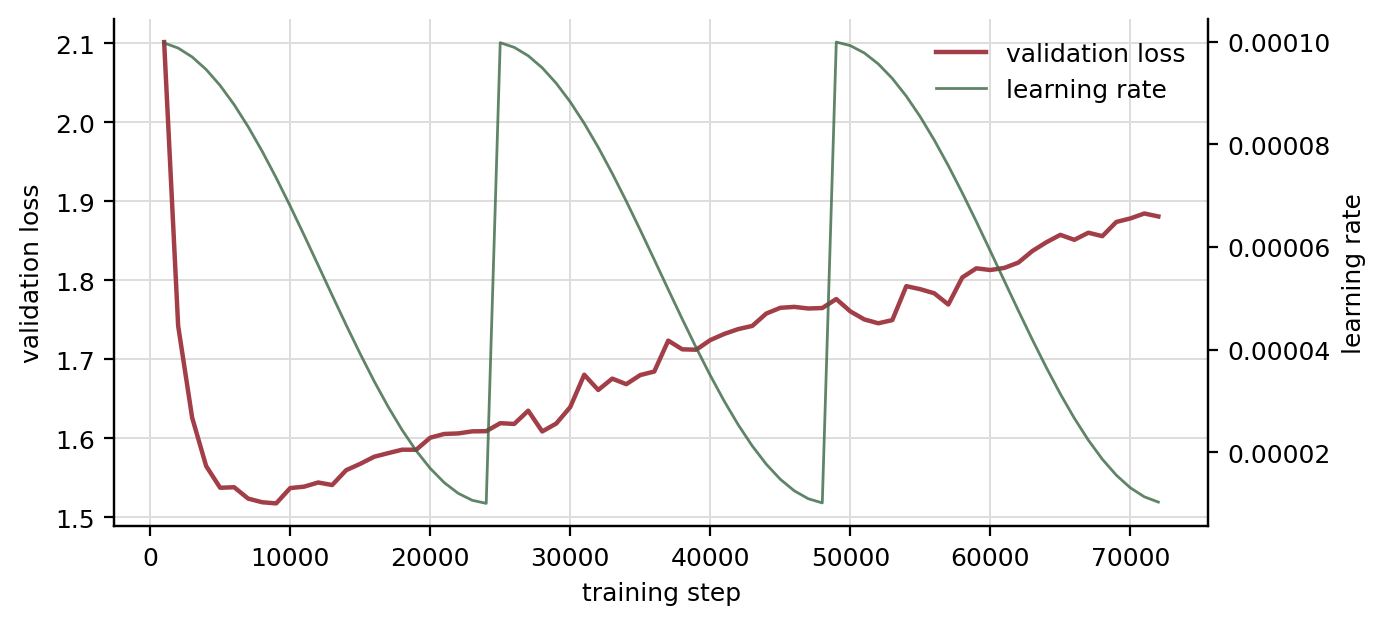
\includegraphics[width=0.90\textwidth]{figures/xlstm_medium_lr_restart_val_curve.png}
	\caption{Validation loss and learning-rate schedule for the medium tokenizer-14 run. The run uses cosine restarts, but its best validation point occurs early, before the first full restart cycle completes.}
	\label{fig:xlstm-medium-lr-restart}
\end{figure}

This final run is therefore best interpreted as a diagnostic follow-up, not as evidence that the medium architecture is unusable. It shows that the selected medium schedule overtrained the current subset.
